%
% ------------------------------------------------------------------------------
\section{The Earthquake Rupture Forecast Calculator}
\index{Seismic Sources!Model}
\index{Seismic Sources!Initial Model}
The \gls{earthquakeruptureforecast} is a fundamental concept in the OpenSHA 
framework \citep{field2003} as well as in the hazard component of OpenQuake.

As discussed in the previous Section, the calculation of the \gls{acr:erf} 
in OQ starts from a \gls{seismicsourcemodel} created by the  
\gls{logictreeprocessor}.
%
When epistemic uncertainty is not included in the \gls{seismicsourcesystem}
there exists a one to one correspondance between the 
\gls{initialseismicsourcemodel} and the \gls{seismicsourcemodel} used 
in the calculation of hazard. In this case, the \gls{logictreeprocessor} 
just duplicates into the \gls{seismicsourcemodel} the information 
included in the \gls{initialseismicsourcemodel}.
%
In more complicated cases, when epistemic uncertainty affects many 
parameters characterizing seismic sources, the \gls{logictreeprocessor} 
generates many \glspl{acr:ssm} so as to explore entirely the space 
of models admitted by our imprecise knowledge.

Independently of the \gls{seismicsourcelogictree} complication,
the Earthquake Rupture Forecast calculator processes one at a time the 
\glspl{acr:ssm} and creates a list of the ruptures generated by all 
the sources in the \gls{acr:erf}. 
%
Each rupture in the list is associated with a probability of occurrence 
in the \gls{investigationtime} specified by the user in the calculation 
settings. To produce this results, the earthquake rupture forecast 
calculator treats separately each source typology included in the 
seismic source model. A detailed description of the methodologies 
adopted to create the earthquake rupture forecast for different seismic
source types is provided in the following Sections.

As a final important note: so far OQ supports just sources 
producing seismicity in accordance with a Possion temporal occurrence 
model.
%
% - - - - - - - - - - - - - - - - - - - - - - - - - - - - - - - - - - - -- - - -
\subsection{ERF creation in case of distributed seismicity}
Open Quake supports two seismic source typologies capable to model 
distributed seismicity: \glspl{areasource} and \glspl{gridsource}.

Area sources are the most traditional source type adopted in PSHA 
analysis since its first introduction at the end of the 1960s. 
%
The works of \cite{frankel1995} and \cite{frankel1997} boosted the 
use of grid sources in probabilistic seismic hazard calculations. 
%
%. . . . . . . . . . . . . . . . . . . . . . . . . . . . . . . . . . . . . . . .
\subsubsection{Area source}
\label{sec:areasource}
%
The creation of an ERF in case of \glspl{areasource} (see also Section 
\ref{hazard:seismic_source_types:areaSources} at page 
\pageref{hazard:seismic_source_types:areaSources}) requires a 
preliminary step consisting in the discretization of the polygon 
used to delimit the spatial extension of the source. 
%
% . . . . . . . . . . . . . . . . . . . . . . . . . . . . . . . . . . . > Figure
\begin{figure}[!ht]
\centering
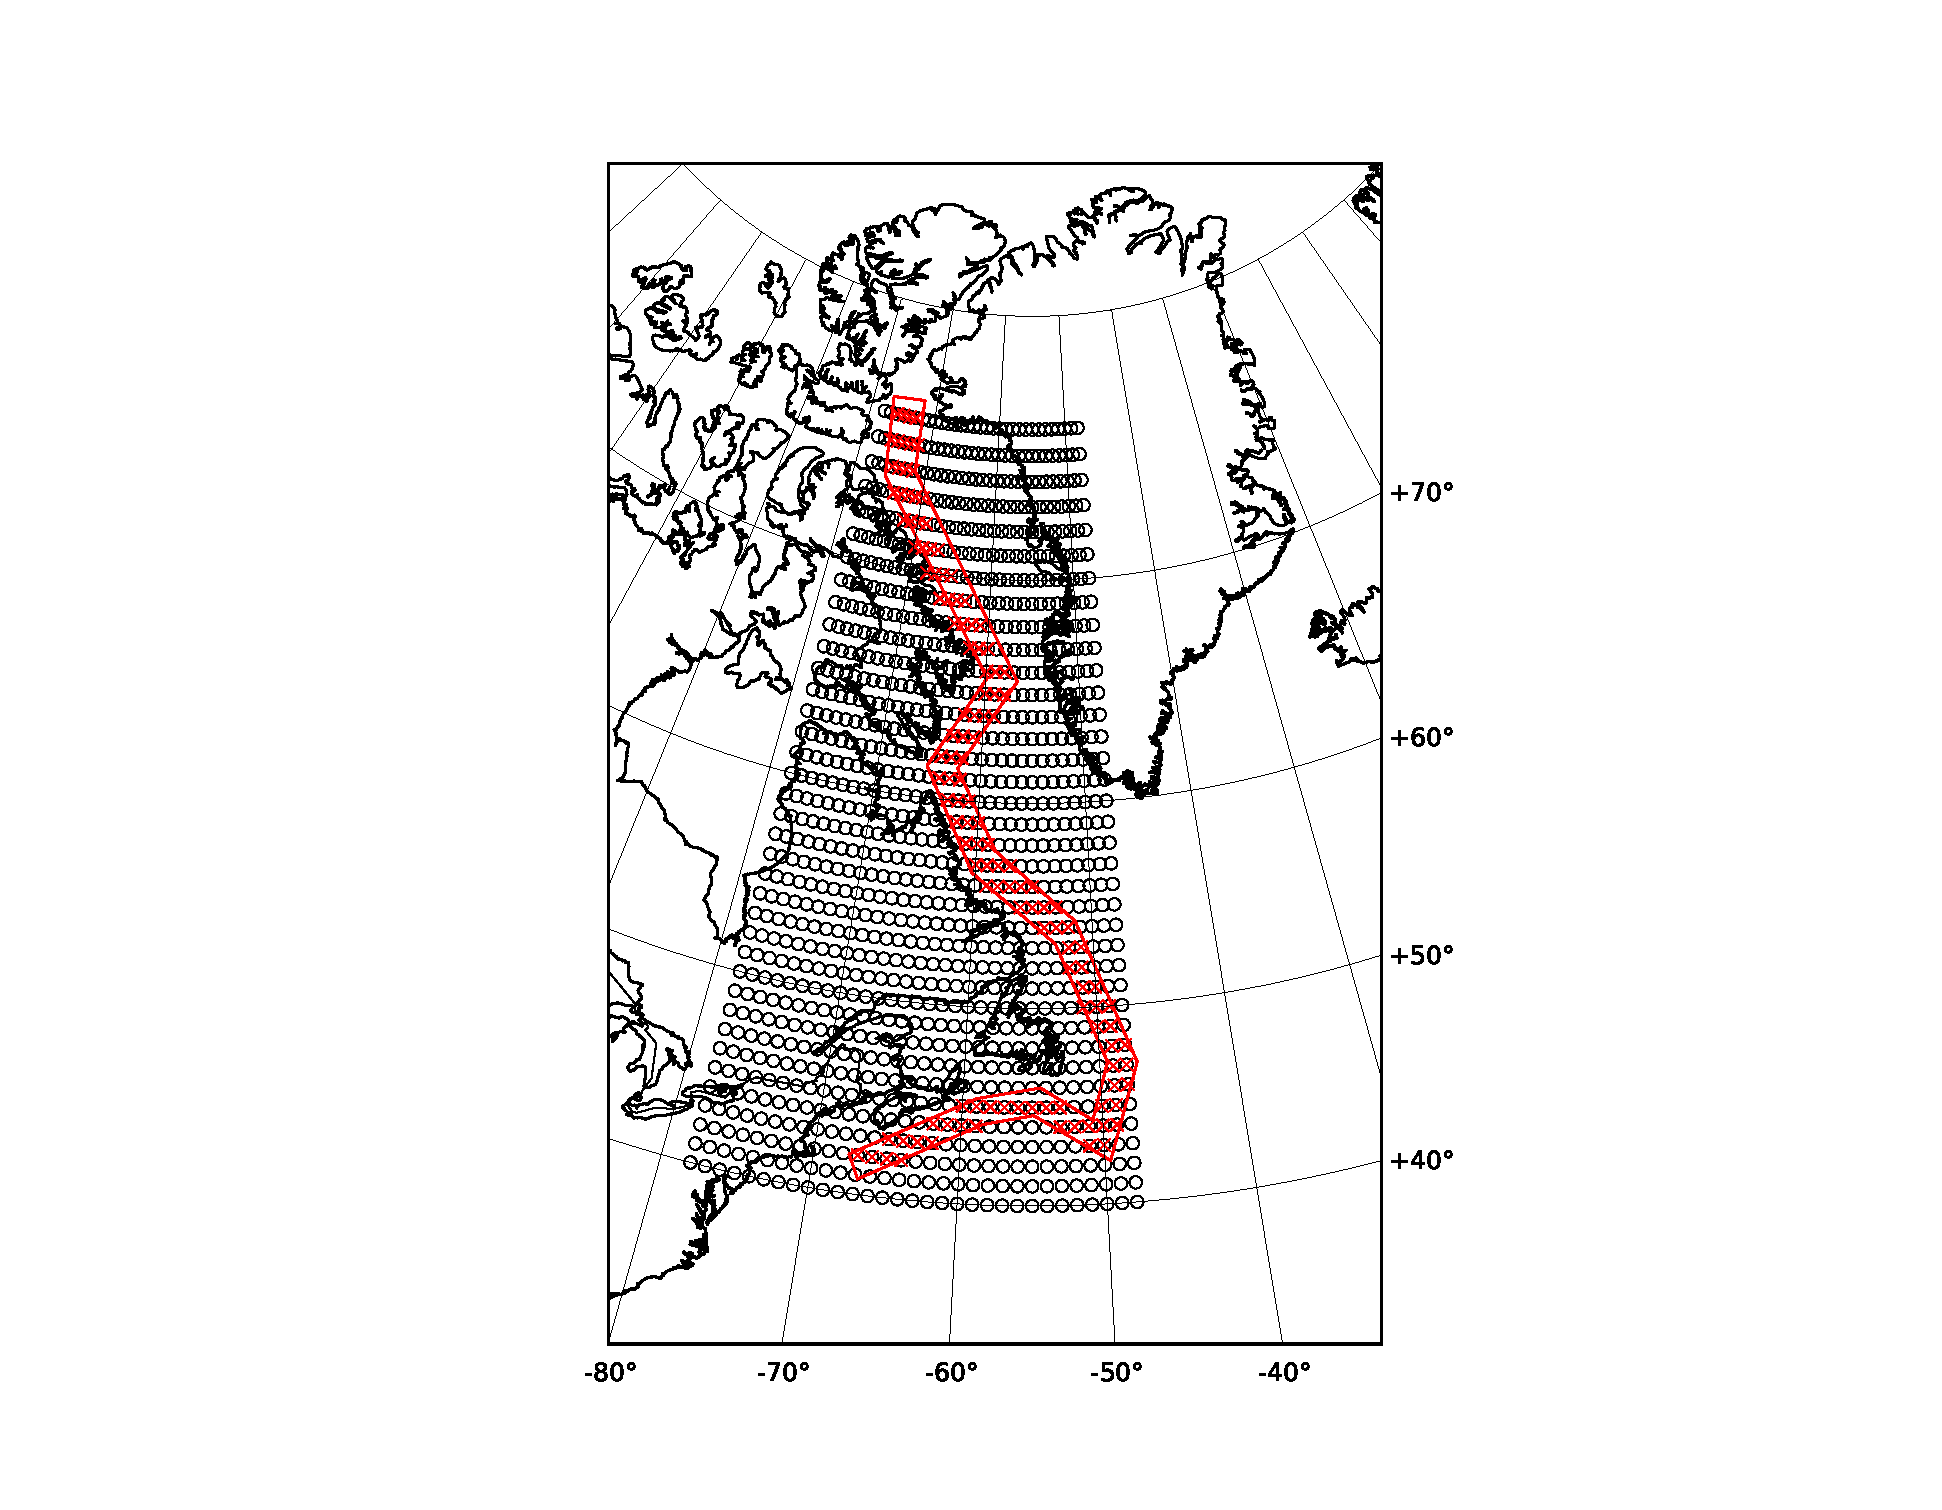
\includegraphics[width=18cm]{./Figures/Part_Hazard/area_source_discretization.eps}
\caption{Example of an area source discretisation (grid spacing equal 
to 0.5$^\circ$). Note how the spacing between circles decreases moving from 
bottom to top of the source.}
\label{fig:area_source_discret}
\end{figure}
% . . . . . . . . . . . . . . . . . . . . . . . . . . . . . . . . . . . < Figure
%
OQ discretizes area sources by overlapping a regular grid of nodes
over the polygon representing the source. The grid contains nodes 
equally spaced in latitude and longitude; the position of each node
is specified by one geographic coordinate, expressed in decimal degrees. 
The nodes of the grid inside the polygon represent - in a discrete way - 
the area source.

The reference system adopted has the advantage that is simple and 
intuitive, however from a computational point of view it has some 
drawbacks. The most relevant one is that the spacing (in km) between 
nodes of the grid depends on latitude. 
%
Indeed, the spacing between two nearby nodes close to the equator is 
larger than at high latitudes e.g. one degree of longitude at the equator 
correponds to about 111 km, at 45$^\circ$ of latitude it becomes 
about 78.8 km and, at 75$^\circ$ it corresponds to only 28 km. 
%
Figure \ref{fig:area_source_discret} shows a discretization example 
considering an area source contained in the Canada model \citep{adams2003}. 
%
If we assume the grid nodes as centers of rectangular cells, the shape
of these cells tends to be squeezed as we move towards the poles.

The problem of this uneven distribution of the cell size arises when we 
distribute the seismicity defined for the entire area source over the 
nodes used to represent its shape. If the node spacing along the 
meridians was homogenous, the seismicity on each node would be 
simply the total seismicity divided by the number of nodes selected 
to discretize the area source.
%
In reality this condition is never satisfied, as a consequence, to 
guarantee a homogeneous distribution of seismicity rates,
we adopt a simple procedure that distributes the seismicity rates 
proportionally to the cell size (i.e grid node spacing).
%
Particularly, for each node of an area source we compute the area using
the following relationship:
\begin{equation}
	a_{node} = 4\pi^2 * spc^2 *  
 	\left(\frac{\text{earth\_radius}}{360}\right)^2 * 
 	\sin(\text{node\_latitude})
\label{eq:cell_area}
\end{equation}
where:
\begin{itemize}
\item $spc$ is the distance between two consecutive cells 
	of the grid adopted to discretize the area source (a common value 
	adopted to discretize sources is equal to 0.1)
\item earth\_radius is the mean radius of the Earth (approximately 
	6371 km) 
\item node\_latitude is the latitude of the cell of which we compute
	the area.
\end{itemize}
%
To get the \glspl{seismicityrate} for a single grid node we multiply the 
ratio between the area (computed using equation \ref{eq:cell_area}) and 
the area of the entire source (i.e. the sum of the areas computed 
with looping for the grid nodes used to discretize the source polygon).
%
% .  .  .  .  .  .  .  .  .  .  .  .  .  .  .  .  .  .  .  .  .  .  .  .  .  .  
\paragraph{ERF calculation}
\label{par:erf_calc_area_src}
In case of a Poissonian temporal occurrence model, the probability of 
occurrence during the investigation time $t$ of a rupture $rup$ with 
magnitude $m$ on node $node$ (belonging to $src$) corresponds to:
\begin{equation}
P(rup_{src}(m_i)|t)=\lambda_{node}(m_i)\,t\exp(-\lambda_{node}(m_i)\,t)
\label{eq:rupture_prob_occ}
\end{equation}
where $\lambda_{node}(m_i)$ is the rate of occurrence of magnitude $m_i$ 
for rupture $rup$ on node $node$. $\lambda_{node}$ is computed as follows:
\[ 
\lambda_{node}(m_i) = \lambda_{src}(m_i)a_{node}/a_{src}
\]
%
where $\lambda_{src}(m_i)$ is the rate of occurrence of magnitude $m_i$
within source $src$, $a_{node}$ is the area of the $node$ computed using
equation \ref{eq:cell_area} and $a_{src}$ is the area of $src$ (it can be
computed by iteratively applying equation \ref{eq:cell_area} to the 
nodes used to represent the $src$ polygon and summing the results). 

The inclusion in the \gls{acr:erf} of the of ruptures produced by 
an area source is an iterative procedure with two nested loops, one 
for the nodes used to discretize the area polygon and the second for 
the magnitude intervals. 
%
During each loop, the probability of occurrence of the rupture $rup$
with magnitude $m_i$ is computed using equation \ref{eq:rupture_prob_occ}.
Eventually, a finite rupture geometry is generated using a magnitude 
scaling relationship. Finally, rupture geometry and $P(rup_{src}(m_i)|t)$
are added to the \gls{acr:erf}.
%
%. . . . . . . . . . . . . . . . . . . . . . . . . . . . . . . . . . . . . . . .
\subsubsection{Multi-depth area source}
%
{\color{blue}{
%
\marginpar{This source typology is not supported by the current version of OQ}
%
This source typology is an extension of the just described 
\gls{areasource} (see page \pageref{sec:areasource});
it allows to distribute seismicity within a volume laterally 
limited by the projection along the depth-axis of a polygon 
lying on the topographic surface and on top and bottom by 
two planes - parallel to the topographic surface - identifying the 
upper and lower seismogenic depths.

The creation of the \gls{acr:erf} in case of multi-depth area sources
follows the same fundamental criteria discussed in the previous section 
for area sources. 
%
The \gls{acr:fmd} for the entire source is distributed over the nodes 
of the 3D grid used to describe the source volume.
%
% .  .  .  .  .  .  .  .  .  .  .  .  .  .  .  .  .  .  .  .  .  .  .  .  .  .  
\paragraph{ERF calculation}
The calculation of the ERF in case of multi-depth area sources follows
the same general concepts described for the area source typology.
%
The processing is based on two nested loops, one for the nodes 
used to discretize the volume and the second for the magnitude intervals. 
}\color{black} % end of textcolor blue
%
%. . . . . . . . . . . . . . . . . . . . . . . . . . . . . . . . . . . . . . . .
\subsubsection{Grid source}
\Glspl{gridsource} are becoming a valuable alternative
to area sources when there's a need for modeling distributed 
seismicity in \gls{acr:psha} \citep{frankel1995}. 
%
The main advantage of \glspl{gridsource} consists on the seismicity 
smoothing procedure usually adopted for their calculation, which appears
to be objective, reproducible and - generally - not particularly complex. 
%
In spite of their simplicity, these source typology must be created 
with extreme care \citep[][page 9]{abrahamson2006}
%
During the latest years an number of regional and national PSHA models 
based on grid sources to account for distributed seismicity were 
published in the literature \citep{stirling2002,petersen2008}. 

%
The current \gls{acr:oq} implementation of this source typology 
uses most of all the \gls{opensha} \texttt{PointEqkSource.java}
and \texttt{PointToLineSource.java} classes.
%
% .  .  .  .  .  .  .  .  .  .  .  .  .  .  .  .  .  .  .  .  .  .  .  .  .  .  
\paragraph{ERF calculation}
The calculation of the \gls{acr:erf} in case of grid sources follows 
the same general concepts described for the area source typology.
The most relevant difference in case of grid sources relates to the 
information about seismicity that changes from node to node.

The inclusion of the ruptures produced by a grid source in the 
\gls{acr:erf} is an iterative procedure with two nested loops, one 
for the nodes of the grid and the second for the magnitude intervals. 
%
%. . . . . . . . . . . . . . . . . . . . . . . . . . . . . . . . . . . . . . . .
\subsubsection{Accounting for rupture finiteness in case of distributed 
seismicity}
% 
The increase - within the last two decades - of the number of 
ground-motion recordings and earthquakes meta-information raised 
the need to appropriately account for the finite dimension of rupture 
in the calculation of hazard.
% 
While this issue does not imply relevant difficulties in case of 
fault sources, different approaches exists to account for rupture 
finiteness in case of seismic sources modelling distributed 
seismicity. 
% 
These approaches reflects distinct thinking of the 
large epistemic uncertainties affecting the potential seismogenic 
structures and the computation demand implied by the likely 
large number of ruptures to process when ruptures are explicitly
considered.

Two are the common approaches adopted to properly take into 
consideration the finite dimension of ruptures in case of sources 
of distributed seismicity.

The first approach uses punctual sources and adjusts the 
rupture-site distance to account for the finite dimension of rupture.
%
This distance correction is usually based on a complete ignorance 
hypothesis implying the use of vertical uniformly spoked ruptures.
%
Such an assumption is in general acceptable but in cases where the 
ground-motion models using a R$_{rup}$ metric and the tectonic context
is characterized by very low dipping sources.
%
For example, \citet{petersen2008} used this solution to calculate
the latest release of the National Seismic Hazard Maps for the 
conterminous United States \citep[see also][]{harmsen2008}. 
%
Rupture-site corrections factors where also proposed by 
\citet{scherbaum2004} and discussed in \citet{beyer2006}.

The second approach uses finite ruptures - centered on each node 
of the grid - either spoked or with random orientation and,  
usually, vertical dip. 
%
In some cases, the generation of ruptures with properties 
restrained to specific seismotectonic styles available for distinct  
geographic contexts is possible. 
%
This approach is generally more computationally intensive than the 
solution based on a source-distance adjustment but - being 
customizable - offers a larger flexibility than precomputed solutions.
%
This approach was used by \citet{frankel2002} to calculate the 2002
version of the United States National Seismic Hazard Maps.
%
%.  .  .  .  .  .  .  .  .  .  .  .  .  .  .  .  .  .  .  .  .  .  .  .  .  .  .
\paragraph{Options available in OpenQuake}
Of the two just approaches just discussed, OpenQuake currently supports 
only the one based on the use of finite ruptures.

The computation of finite ruptures in \gls{acr:oq} follows a unified 
procedure for area, multi-depth and grid sources since each node
of the grid used in the different cases has always one or several 
sets containing the following information:
%
\begin{itemize}
\item A discrete representation of a \gls{acr:fmd} 
\item A faulting style: strike [optional], dip [optional] and rake 
[optional] 
\end{itemize}
%
The definition of one, or several, faulting styles is optional; the 
simplest case - using on compulsory information - is based on the 
knowledge of just one discrete FMD.
%
% . . . . . . . . . . . . . . . . . . . . . . . . . . . . . . . . . . . > Figure
\begin{figure}[!hb]
\centering
\includegraphics[width=13cm]{./Figures/Part_Hazard/area_source_finite_ruptures.eps}
\caption{Example of random ruptures generated with OpenQuake to take 
into account rupture finiteness in case of hazard computation based 
on a single area source.}
\label{fig:area_source_finite_ruptures}
\end{figure}
% . . . . . . . . . . . . . . . . . . . . . . . . . . . . . . . . . . . < Figure
%

Different approaches are available to account for finite ruptures;
their adoption depends on the information provided by the user on
the specific requirements of the analysis and the computational demand
sustainable. 
%
These are the main options available:
\begin{itemize}
	\item Generate ruptures aligned according to a specified faulting style 
	(this approach can be used when at least the strike direction is 
	specified)
	\item Random ruptures 
	\item Crosshair ruptures
	\item Spoked rupture
\end{itemize}
The last three options are always applicable since compulsory information 
suffices.
%
% - - - - - - - - - - - - - - - - - - - - - - - - - - - - - - - - - - - - - - - 
\subsection{ERF creation in case of Fault sources}
\gls{acr:oq} currently supports two types of fault sources that 
differ at most in the geometry of the fault surface. 
%
Fault sources with a simple geometry are usually utilized to model 
shallow sources while fault sources with a complex geometry are 
better suited to model subduction interface sources.
%
%. . . . . . . . . . . . . . . . . . . . . . . . . . . . . . . . . . . . . . . .
\subsubsection{Fault sources with simple geometry}
%
The current \gls{acr:oq} implementation of this source typology 
corresponds to the one included in the \gls{opensha}
\texttt{FloatingPoissonFaultSource.java} class.

In \gls{acr:oq}, \glspl{simplefaultsource} represents tectonic structures 
with a straightforward geometry characterized by relatively constant 
values of dip over the entire surface and along-strike profiles at 
different depths similar to the fault trace. 

The methodology used for the creation of the fault surface takes the 
fault trace, a representative dip direction (e.g. it could be the mean 
dip direction) and, the upper and lower seismogenic depth and creates 
a 3D gridded surface using a number of equally spaced nodes. 
%
%. . . . . . . . . . . . . . . . . . . . . . . . . . . . . . . . . . . . . . . .
\subsubsection{Fault sources with complex geometry}
%
The \gls{acr:oq} implementation of this source typology at the moment 
uses most of all the \gls{opensha} \texttt{FloatingPoissonFaultSource.java}
and \texttt{ApproxEvenlyGriddedSurface.java} classes.

Fault sources with complex geometry tries to replicate the geometry of
subduction interfaces \citep{hayes2009,heuret2011}.
Because of the methodology used to create the source and float the 
ruptures on its surface this seismic source typology has a major 
drawback which corresponds to an in-homogenous density of seismic 
moment released per unit of surface (i.e. the rupture area for a specific
magnitude varies over the fault surface).
%
%. . . . . . . . . . . . . . . . . . . . . . . . . . . . . . . . . . . . . . . .
\subsubsection{Computing the probability of occurrence of each rupture}
In case of sources with a Poissonian \gls{temporaloccurrencemodel}, the 
probability of occurrence for a given rupture - that equals the probability
of occurrence of corresponding magnitude, given a magnitude scaling
relationship - is computed using a procedure that's conceptually 
homologous with the one described in case of \glspl{areasource} (see
page \pageref{par:erf_calc_area_src}). 

In this case, the main difficulty is related to the calculation - given a 
magnitude interval - arises when ruptures with a surface smaller than the 
entire fault are allowed to float. In this case finite ruptures are 
homogeneously distributed over the fault surface and the rate of occurrence
for each rupture (i.e. magnitude) is computed as the ratio between the number 
in order to derive the 
rate of occurrence. 
